\documentclass[tikz,border=0pt]{standalone}
\usepackage{pgfplots}
\usepackage{xcolor}

\begin{document}
\begin{tikzpicture}
\begin{scope}
    \node[inner sep=0pt]  at (0,0)
        {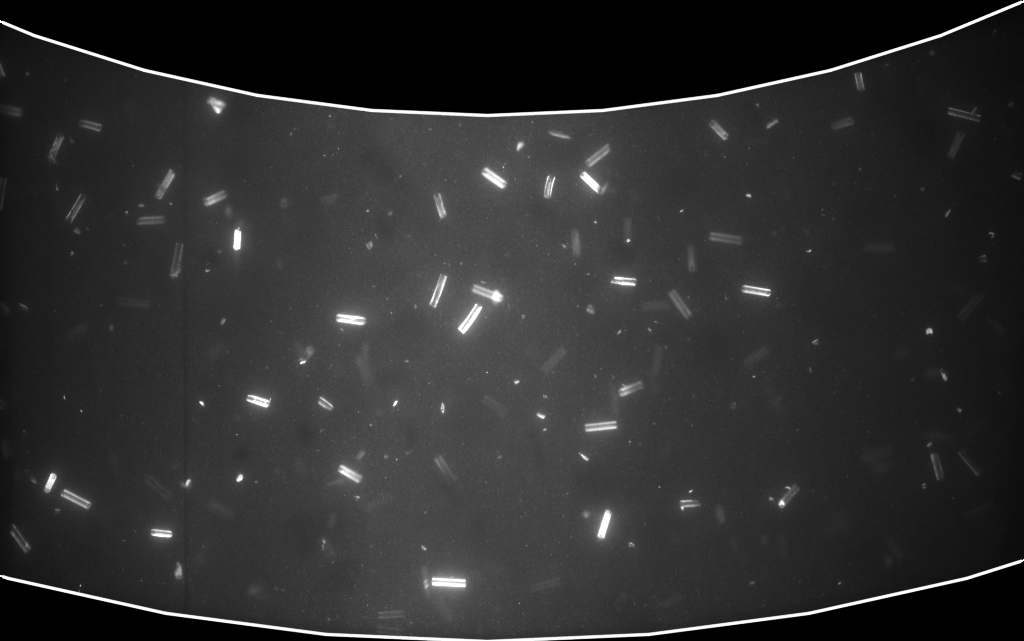
\includegraphics[height=7cm]{stillimage.png}};
\end{scope}

\begin{scope}[
    xshift=6.cm,
    yshift=4.0cm
    ]

\end{scope}
    
% labels
\node at (-3.6, 3.25) {(a)};
\node at (3.65, 3.25) {(b)};
\node at (3.65, -0.50) {(c)};

\end{tikzpicture}
\end{document}
